\documentclass[11pt,a4paper]{article}
\usepackage[utf8]{inputenc}
\usepackage[T1]{fontenc}
\usepackage{amsfonts}
\usepackage[french]{babel}
\frenchbsetup{StandardLists=true} % à inclure si on utilise \usepackage[francais]{babel}
\usepackage{enumitem}
\usepackage{amssymb}
\usepackage{amsmath}
\usepackage[left=2cm,right=2cm,top=2cm,bottom=2cm]{geometry}
\usepackage{multirow}
\usepackage[dvipsnames]{xcolor}

\usepackage[T1]{fontenc}
\usepackage{fouriernc}
\usepackage{graphicx}

\usepackage{setspace}
\singlespacing

\usepackage{pstricks}
\usepackage{xkeyval}
\usepackage{pst-labo}


\usepackage{multicol}
\usepackage{caption}
\usepackage{fancyhdr}
\pagestyle{fancy}
\renewcommand\headrulewidth{1pt}
\fancyhead[L]{Lycée Denis Diderot }
\fancyhead[R]{Classe de Première Bac Pro}
\setcounter{page}{4}\fancyfoot[C]{page \thepage}
\fancyfoot[R]{Année 2025-2026}
\fancyfoot[L]{Alexis RUIZ}
\usepackage{multirow,tabularx,booktabs}
\newcommand{\cadreblanc}[1]{%
\medskip\framebox[\linewidth][c]{%
\rule{0mm}{#1mm}}\par
\medskip}

\usepackage{awesomebox}
\setlength{\aweboxvskip}{0mm}
\usepackage{pifont}
\usepackage{chemmacros}
\chemsetup{modules=all}
\setlength{\columnseprule}{.25mm}

\renewcommand{\arraystretch}{2}
\newcommand*\acocher{\quitvmode{\fboxsep0pt \fboxrule0.8pt \fbox{\vrule height1.8ex depth.1ex width0pt \vrule height0pt depth0pt width1.9ex }}}

\newcommand{\code}{\awesomebox[black]{2pt}{

\includegraphics[scale=0.15]{images/frame.png}
}{black}}

\newcommand{\moteur}{\awesomebox[black]{2pt}{

\includegraphics[scale=1]{images/moteur.jpg} 
}{black}}

\newcommand{\defconclusion}{\awesomebox[black]{2pt}{\rotatebox{90}{\Large{\textbf{Conclusion}}}}{black}}

\usepackage[tikz]{bclogo} 
\newcommand{\ctext}[1]
{\begin{bclogo}[couleur = white,logo= , arrondi = 0.1,barre=none]
{}
\vspace{-8mm}
~~
\textcolor{red}{#1}
~~
\end{bclogo}}



\frenchbsetup{StandardLists=true}



\begin{document}


\flushleft \textbf{NOM :\\
Prénom:\\[0,4cm]
}
\hrule\
\\[0,2cm]




\begin{center}
 \LARGE{Activité 2 - Quelle est l'énergie électrique reçue ?  }
\end{center}



\normalsize

\hrule\
\\[0,2cm]
   \begin{center}
   \textbf{Le soin et la rédaction interviendront dans la notation.}
   \end{center} 

\noindent%
\begin{minipage}{.8\textwidth}%
 
  Sur la fiche technique d'une perceuse-visseuse sans fil sont notées les information suivantes : 
  \begin{itemize}
      \item moteur électrique : $P=27\ W$ et $I=1,5\  A$
      \item accumulateur : $U = 18\ V$ et capacité : $I \times t_{max}=2\ A.h$
  \end{itemize}

\end{minipage}%
\hfill
\begin{minipage}{.15\textwidth}%
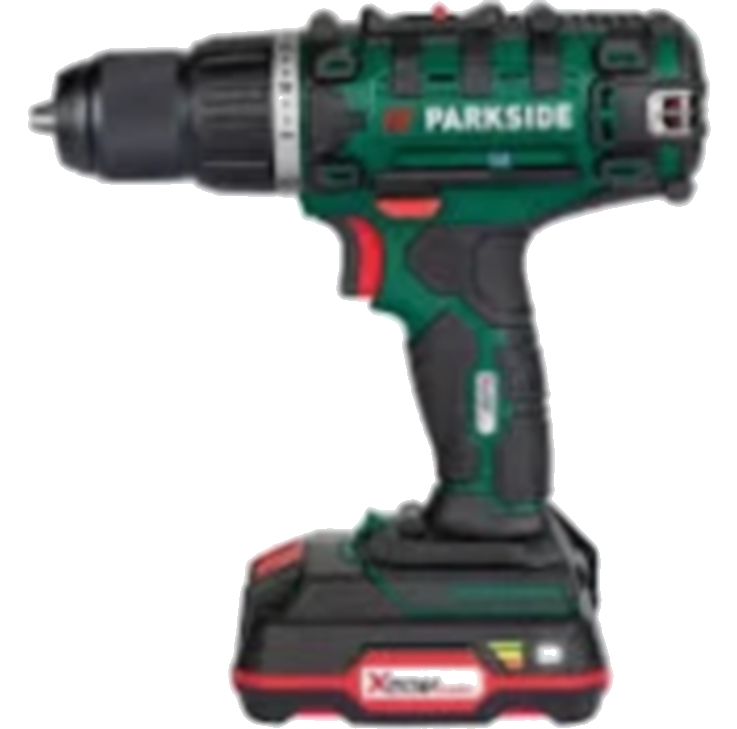
\includegraphics[width=\textwidth]{images/A2 - perceuse.jpg}
\end{minipage}%

\vspace{5mm}

  \ding{202} Calculer, en heure puis en seconde, la durée maximale $t_{max}$ de fonctionnement de la perceuse alimentée en courant continu par la batterie. \\
  \cadreblanc{10}

  \ding{203} Calculer l'énergie électrique $E$, en Wh puis en J, reçue par le moteur en courant continu durant ce temps $t_{max}$. \\
  \cadreblanc{10}
   
\vspace{1mm}
  \awesomebox[black]{1pt}{\faCogs}{black}{On pourra utiliser les relations suivantes $1W.h = 1W \times 1h $ et $1J = 1W \times 1s$}
\vspace{1mm}

  
\hrule\


\begin{center}
 \LARGE{Activité 3 - Comment faut-il brancher l'ampèremètre et le voltmètre ?   }
\end{center}

\normalsize

\hrule\

\vspace{3mm}
\noindent%
\begin{minipage}{.65\textwidth}%
 
 \ding{202} Identifiez les grandeurs et unités électriques nominales de la lampe torche à diode électroluminescente correspondant aux conditions optimales de fonctionnement [Doc.1]

\cadreblanc{8}

\ding{203} En vous servant des valeurs, rechercher une relation mathématique entre $I$,  $U$ et $P$.\\
\cadreblanc{8}

\ding{204} Dessiner le schéma électrique du montage du Doc.2 qui modélise la lampe. Ajouter un voltmètre en dérivation pour mesurer la tension aux bornes de la DEL et un ampèremètre en série pour mesurer le courant traversant la DEL. 

\cadreblanc{25}

\end{minipage}%
\hfill
\begin{minipage}{.3\textwidth}%
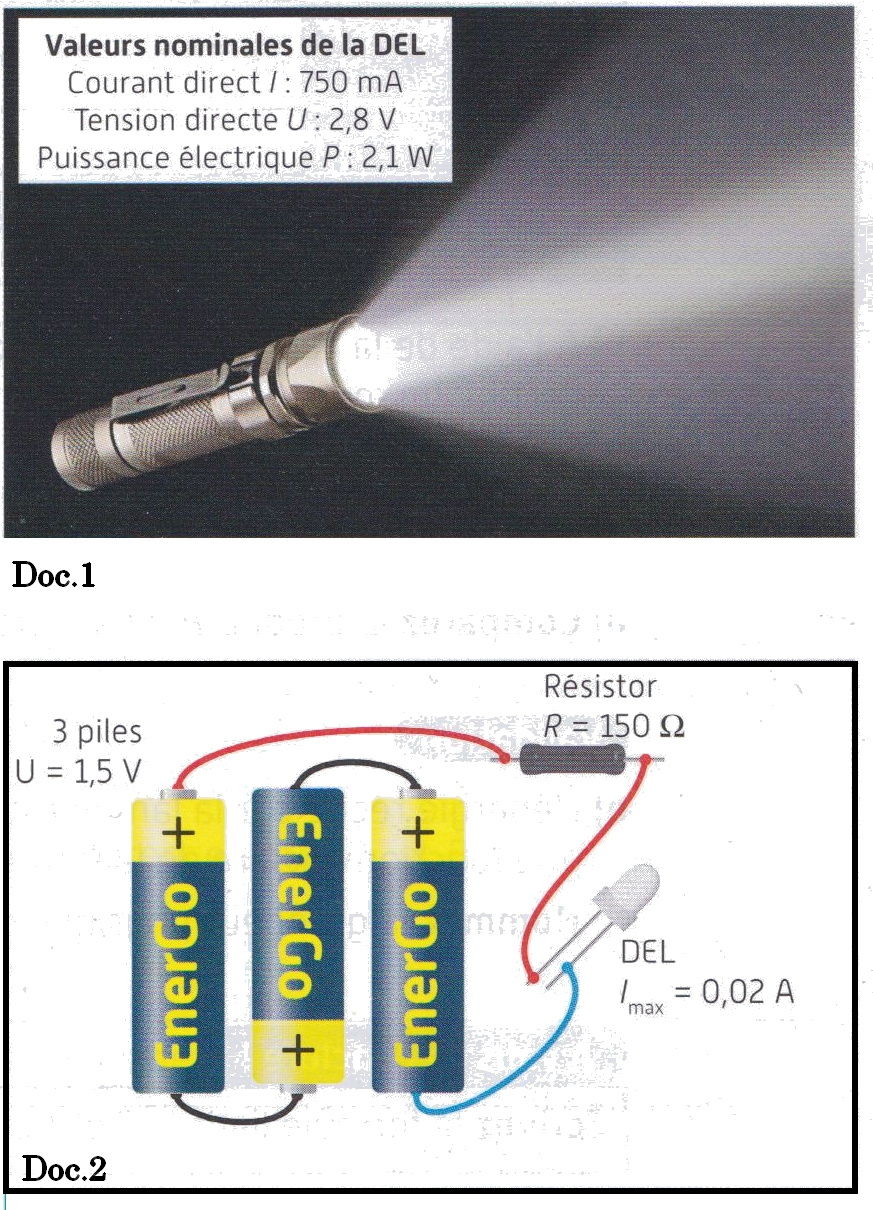
\includegraphics[width=\textwidth]{images/A3.jpg}
\end{minipage}%

\end{document}